\documentclass[11pt]{article}

% --- packages ---
\usepackage[margin=1in]{geometry}
\usepackage{amsmath,amssymb,amsfonts}
\usepackage{booktabs}
\usepackage{graphicx}
\usepackage{hyperref}
\usepackage{xcolor}
\usepackage{multirow}
\usepackage{float}
\usepackage[numbers]{natbib}
\usepackage{algorithm}
\usepackage{algorithmic}
\usepackage{microtype}
\usepackage{bookmark}

\hypersetup{
  colorlinks=true,
  linkcolor=blue!60!black,
  citecolor=blue!60!black,
  urlcolor=blue!60!black
}

% --- metadata ---
\title{%
  La forma della cella:\\
  Confronto empirico delle topologie reticolari cubica e FCC\\
  in teoria dei grafi, operazioni spaziali, elaborazione del segnale\\
  e recupero di embedding%
}

\author{%
  Timothy Paul Bielec\thanks{Autore corrispondente: \texttt{timothy@promptcrafted.com}}\\
  Promptcrafted LLC\\
  Los Angeles, CA
}

\date{Marzo 2026}

\begin{document}

\maketitle

% ===================================================================
\begin{abstract}
Le griglie cubiche costituiscono la discretizzazione predefinita nei sistemi
computazionali---immagini, volumi e strutture dati spaziali.

Questo articolo presenta un confronto empirico sistematico tra il reticolo
cubico semplice (SC, 6-connesso) e il reticolo cubico a facce centrate (FCC,
12-connesso) in quattro domini indipendenti: teoria dei grafi, operazioni
spaziali, elaborazione del segnale e recupero di embedding ad alta
dimensionalit\`a. A ogni scala testata (125--8{,}000 nodi), il reticolo FCC
offre vantaggi di instradamento (percorsi pi\`u brevi del 30\%), guadagni
in robustezza (connettivit\`a algebrica 2,4$\times$, diametro ridotto del
40\%), miglioramenti nella fedelt\`a del segnale (errore di ricostruzione
4--10$\times$ inferiore) e benefici nel recupero (+15--26 punti percentuali
di recall degli embedding a 1-hop). Il costo \`e limitato: approssimativamente
$2\times$ il numero di archi ($12/6$). A tutte le scale testate, questi
rapporti sono stabili, il che suggerisce che il vantaggio derivi dalla
geometria della cella piuttosto che dalla dimensione del campione. Una
libreria open-source (\texttt{rhombic}) e una demo interattiva riproducono
ogni risultato.
\end{abstract}

\noindent\textbf{Parole chiave:} topologia reticolare, cubico a facce centrate,
dodecaedro rombico, teoria dei grafi, elaborazione del segnale, recupero di
embedding, strutture dati spaziali, ricerca approssimata del vicino pi\`u
prossimo

% ===================================================================
\section{Introduzione}
\label{sec:intro}

Il reticolo cubico---espressione spaziale della geometria cartesiana---\`e
il riferimento predefinito ampiamente adottato nel calcolo digitale. La
memoria \`e lineare, le griglie di pixel sono quadrate e gli spazi voxel
sono cubici. Questa convenzione si allinea con la geometria analitica
cartesiana (Descartes, 1637) e con le architetture a programma
memorizzato, consolidandosi per convenzione piuttosto che per ottimalit\`a
dimostrata. Riportiamo inoltre scenari in cui il reticolo cubico mantiene
dei vantaggi, tra cui carichi di lavoro allineati agli assi e interrogazioni
ad alta intensit\`a enumerativa (Sezione~\ref{sec:discussion}).

Il reticolo cubico a facce centrate (FCC) realizza l'impacchettamento
sferico pi\`u denso in tre dimensioni (insieme all'HCP; congettura di
Keplero, dimostrata da Hales, pubblicata nel 2005~\cite{hales2005};
verificata formalmente nel 2014--2017~\cite{hales2017}). Le sue celle
di Voronoi sono \textbf{dodecaedri rombici}---poliedri a 12 facce che
tassellano $\mathbb{R}^3$ senza lacune. Laddove ogni cella cubica
condivide facce con 6 vicini, ogni dodecaedro rombico ne condivide con
12. Il reticolo FCC si presenta nelle strutture cristalline (Cu, Al, Au)
poich\'e i sistemi fisici adottano comunemente disposizioni a
impacchettamento denso. Petersen e Middleton~\cite{petersen1962} hanno
stabilito la teoria del campionamento reticolare ottimale in
$\mathbb{R}^N$. Conway e Sloane~\cite{conway1999} ne hanno documentato
estesamente le propriet\`a matematiche.

Nonostante questi risultati consolidati, il reticolo FCC ha visto
un'adozione minima nella pratica computazionale. A nostra conoscenza,
nessuna suite di benchmark sistematica ha confrontato le due topologie
nell'intera gamma di carichi di lavoro serviti dalle strutture dati
spaziali. Questo articolo colma tale lacuna con esperimenti riproducibili
in quattro domini, implementati in una libreria Python open-source.

\subsection{Contributi}

\begin{enumerate}
  \item Un framework di confronto a scala corrispondente che mantiene
    fisso il protocollo di benchmark confrontando i reticoli SC e FCC a
    conteggi di nodi simili, con conteggi esatti riportati per ogni
    metrica (Sezione~\ref{sec:method}).
  \item Benchmark riproducibili in teoria dei grafi
    (Sezione~\ref{sec:graph}), operazioni spaziali
    (Sezione~\ref{sec:spatial}), elaborazione del segnale
    (Sezione~\ref{sec:signal}) e recupero di embedding
    (Sezione~\ref{sec:embed}).
  \item Un indice ANN organizzato in FCC come prova di concetto che
    dimostra il vantaggio topologico su embedding ad alta dimensionalit\`a
    (Sezione~\ref{sec:index}).
  \item Una libreria open-source, \texttt{rhombic}, con 256 test
    e piena riproducibilit\`a (\texttt{pip~install~rhombic}).
\end{enumerate}

% ===================================================================
\section{Contesto e lavori correlati}
\label{sec:background}

\subsection{Geometria reticolare}

Un \textbf{reticolo} in $\mathbb{R}^3$ \`e un sottogruppo discreto
generato da tre vettori di base linearmente indipendenti. Il
\textbf{reticolo cubico semplice} (SC) utilizza la base standard
$\{e_1, e_2, e_3\}$; ogni nodo ha 6 vicini con facce condivise.
Il \textbf{reticolo cubico a facce centrate} (FCC) aggiunge le
traslazioni dei centri di faccia $\{\frac{1}{2}(e_i + e_j)\}$ per
$i \neq j$; ogni nodo interno ha 12 vicini a distanza uguale
$a/\sqrt{2}$ dove $a$ \`e la lunghezza del lato della cella
convenzionale.

La cella di Voronoi del reticolo SC \`e il cubo. La cella di Voronoi
del reticolo FCC \`e il dodecaedro rombico---un poliedro convesso con
12 facce rombiche congruenti, 14 vertici (8 di valenza 3 e 6 di valenza
4) e 24 spigoli. \`E il duale del cubottaedro e una proiezione
dell'ipercubo quadridimensionale~\cite{coxeter1973}. La
Figura~\ref{fig:voronoi} illustra entrambe le celle di Voronoi con la
rispettiva connettivit\`a di vicinato.

\begin{figure}[t]
\centering
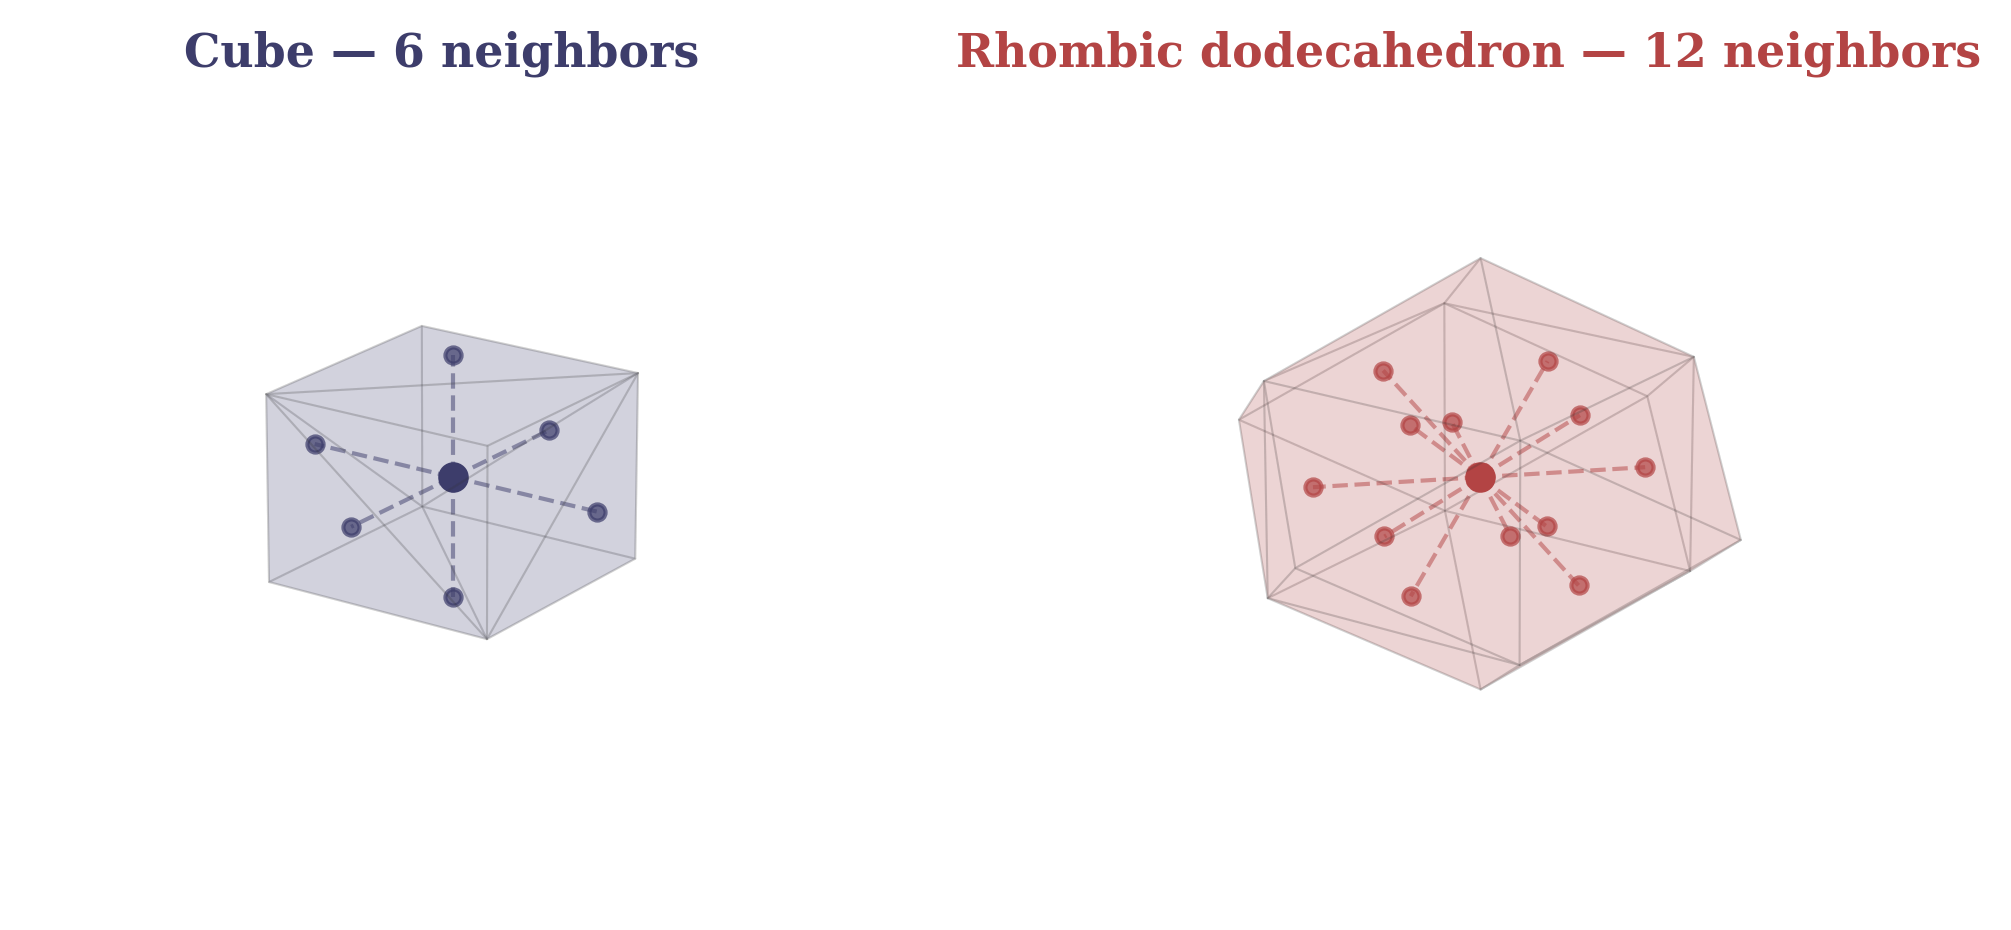
\includegraphics[width=\textwidth]{figures/fig1-voronoi-cells}
\caption{Celle di Voronoi dei reticoli SC e FCC. A sinistra: il cubo
  (6 vicini con facce condivise lungo gli assi coordinati). A destra:
  il dodecaedro rombico (12 vicini con facce condivise nelle direzioni
  diagonali). Le linee tratteggiate indicano la connettivit\`a di
  vicinato; i punti indicano le posizioni dei vicini.}
\label{fig:voronoi}
\end{figure}

\subsection{Impacchettamento sferico e campionamento del segnale}

Keplero congettur\`o (1611) che il reticolo FCC realizza
l'impacchettamento pi\`u denso di sfere uguali, con frazione di
impacchettamento $\pi/(3\sqrt{2}) \approx 0{,}7405$. Sia FCC che HCP
(esagonale a impacchettamento denso) raggiungono questa densit\`a.
Hales dimostr\`o la congettura (pubblicata nel 2005~\cite{hales2005};
verificata formalmente nel 2014--2017~\cite{hales2017}).

Nella teoria del campionamento reticolare 3D, l'ottimalit\`a si formula
nel reticolo reciproco (dominio della frequenza). Petersen e
Middleton~\cite{petersen1962} hanno stabilito il framework generale;
il risultato comunemente citato nella letteratura sulla resa volumetrica
identifica il reticolo BCC come la geometria di campionamento pi\`u
efficiente per limiti di banda isotropi, richiedendo ${\sim}29{,}3\%$
campioni in meno rispetto all'SC a fedelt\`a
comparabile~\cite{theussl2002orvs,theussl2001}. I reticoli FCC e BCC
sono duali reciproci---i loro ruoli si invertono tra spazio reale e
spazio delle frequenze.

I nostri esperimenti valutano l'FCC nel dominio \emph{spaziale} poich\'e
questo lavoro testa una singola topologia su tutti i livelli (grafo,
spaziale, segnale ed embedding) e l'FCC \`e la controparte spaziale
naturale: \`e l'impacchettamento sferico pi\`u denso, la sua cella di
Voronoi (il dodecaedro rombico) fornisce una cella di riempimento dello
spazio altamente isotropa---il suo quoziente isoperimetrico supera quello
del cubo, e lavori precedenti identificano le celle di Voronoi FCC e BCC
come massimi locali tra le tassellazioni di riempimento dello
spazio~\cite{conway1999}---e la sua struttura di grafo 12-connessa
produce i vantaggi di instradamento e propagazione misurati nei
Livelli~1--2. Il Livello~3 (Sezione~\ref{sec:signal}) misura direttamente
il campionamento spaziale FCC con un ricostruttore agnostico rispetto
alla topologia, piuttosto che derivare previsioni dalla teoria del
campionamento. Un baseline BCC \`e un naturale prossimo controllo per
isolare i contributi della teoria del campionamento.

\subsection{Strutture dati reticolari}

L'adozione pratica di reticoli non cubici rimane limitata.
Theu{\ss}l et al.~\cite{theussl2001} hanno dimostrato la
voxelizzazione FCC e BCC per la resa volumetrica.
Csebfalvi~\cite{csebfalvi2010} ha esplorato il campionamento BCC per
l'imaging medico. Entezari et al.~\cite{entezari2004} hanno
formalizzato le box spline BCC per la ricostruzione del segnale.
Tuttavia, nessun lavoro precedente presenta un benchmark sistematico e
multidominio che confronti le topologie SC e FCC a conteggi di nodi
corrispondenti con codice pubblicamente disponibile.

% ===================================================================
\section{Metodologia}
\label{sec:method}

\subsection{Costruzione del reticolo}

Entrambi i reticoli sono costruiti per riempire un volume cubico
delimitante con conteggi di nodi approssimativamente corrispondenti.

\textbf{Reticolo cubico.} $n^3$ nodi posizionati a coordinate intere
$\{0, 1, \ldots, n{-}1\}^3$. Ogni nodo interno si connette ai suoi
6 vicini con facce condivise (vicinato di von Neumann). Numero di archi:
$3n^2(n-1)$.

\textbf{Reticolo FCC.} Ogni cella unitaria cubica convenzionale contiene
quattro siti di base a coordinate frazionarie $(0,0,0)$,
$(\tfrac{1}{2},\tfrac{1}{2},0)$, $(\tfrac{1}{2},0,\tfrac{1}{2})$ e
$(0,\tfrac{1}{2},\tfrac{1}{2})$. Con $n$ celle unitarie per lato, il
reticolo contiene esattamente $4n^3$ nodi. Ogni nodo interno si connette
ai suoi 12 vicini pi\`u prossimi utilizzando i vettori di offset FCC:
\begin{equation}
  \left\{\tfrac{1}{2}(\pm e_i \pm e_j) : 1 \leq i < j \leq 3\right\}
\end{equation}
producendo 12 archi per nodo interno.

\textbf{Corrispondenza.} Per un obiettivo di $N$ nodi, poniamo
$n_{\mathrm{SC}} = \mathrm{round}(N^{1/3})$ (ottenendo
$n_{\mathrm{SC}}^3$ nodi SC) e
$n_{\mathrm{FCC}} = \mathrm{round}((N/4)^{1/3})$ (ottenendo
${\sim}4 n_{\mathrm{FCC}}^3$ nodi FCC dopo deduplicazione).
I due conteggi non sono identici---SC produce cubi esatti mentre
FCC produce conteggi approssimati---pertanto riportiamo i conteggi
esatti dei nodi a fianco di ogni metrica. A tutte le scale qui
riportate, i conteggi differiscono per meno del 15\%.

\subsection{Software e riproducibilit\`a}

Tutti gli esperimenti utilizzano la libreria \texttt{rhombic} (Python
3.10+, dipendenze: NumPy, NetworkX, SciPy). I grafi sono costruiti come
oggetti \texttt{Graph} di NetworkX. L'intera suite di benchmark si
riproduce tramite:
\begin{verbatim}
  pip install rhombic && python -m rhombic.benchmark
\end{verbatim}
Hardware: Windows 11, CPU Intel (i benchmark di grafo/spaziali sono
limitati dalla CPU), NVIDIA RTX 6000 Ada 48\,GB (non utilizzata per
questi benchmark). Codice sorgente, dati grezzi e demo interattiva sono
pubblicamente disponibili (si veda Disponibilit\`a,
Sezione~\ref{sec:conclusion}).

\paragraph{Riproducibilit\`a.}
Tutte le operazioni stocastiche (punti di valutazione del segnale,
generazione di embedding, rimozione casuale di nodi per la tolleranza ai
guasti) utilizzano un seme fisso ($\mathtt{seed}=42$). I benchmark di
teoria dei grafi (Livello~1) e le operazioni spaziali (Livello~2) sono
completamente deterministici data la costruzione del reticolo. I
benchmark del segnale (Livello~3) utilizzano una singola prova per
combinazione frequenza-scala con punti di valutazione fissi. I benchmark
degli embedding (Livello~4) utilizzano una singola prova con generazione
di cluster fissa. Tutti i risultati sono riprodotti da
\texttt{python~-m~rhombic.benchmark} dalla release \texttt{v0.1.2}
(\texttt{pip install rhombic==0.1.2}). L'artefatto PyPI include
un'attestazione di provenienza che collega il pacchetto pubblicato
al commit del repository sorgente.\footnote{Differenze di virgola mobile
tra piattaforme possono produrre variazioni alla cifra meno significativa;
tutti i rapporti qui riportati sono stabili sulle piattaforme testate
(Windows~11/Linux, Python~3.10--3.12).}

% ===================================================================
% Transizione: dalla motivazione geometrica alla misura empirica
\section{Livello 1: Teoria dei grafi}
\label{sec:graph}

Riportiamo ora le misure empiriche: ogni livello definisce un benchmark
a scala corrispondente e riporta i rapporti beneficio-costo osservati.

Misuriamo quattro propriet\`a di teoria dei grafi a tre scale
(125--4{,}000 nodi). Tutte le metriche sono calcolate sui grafi
reticolari completi tramite NetworkX.

\subsection{Metriche}

\textbf{Lunghezza media del cammino minimo} (ASPL): media su tutte le
coppie di nodi, calcolata tramite BFS. \textbf{Diametro}: cammino minimo
massimo. \textbf{Connettivit\`a algebrica}: secondo autovalore pi\`u
piccolo del laplaciano del grafo (valore di
Fiedler~\cite{fiedler1973}). \textbf{Tolleranza ai guasti}: frazione di
nodi raggiungibili dalla componente connessa pi\`u grande dopo la
rimozione del 10\% dei nodi in modo uniforme casuale.

\subsection{Risultati}

\begin{table}[H]
\centering
\caption{Benchmark di teoria dei grafi. Tutti i rapporti di vantaggio
${>}\,1$ indicano prestazioni superiori dell'FCC; il rapporto degli archi
\`e il costo.}
\label{tab:graph}
\begin{tabular}{lrrrrrr}
\toprule
Scala & Nodi (SC/FCC) & SC ASPL & ASPL$^a$ & Diam.$^a$
  & Conn.\ alg.$^b$ & Costo archi$^b$ \\
\midrule
${\sim}125$  & 125 / 108   & 4,84 & 1,45$\times$
  & 1,71$\times$ & 2,31$\times$ & 1,50$\times$ \\
${\sim}1000$ & 1000 / 864  & 9,91 & 1,46$\times$
  & 1,69$\times$ & 2,55$\times$ & 1,61$\times$ \\
${\sim}4000$ & 4096 / 4000 & 15,94 & 1,40$\times$
  & 1,61$\times$ & 2,43$\times$ & 1,88$\times$ \\
\bottomrule
\multicolumn{7}{l}{\footnotesize $^a$SC/FCC (pi\`u breve~=~migliore).
$^b$FCC/SC.}
\end{tabular}
\end{table}

Il vantaggio di ASPL \`e stabile al 29--32\% a tutte le scale testate
(Figura~\ref{fig:benchmarks}). Il rapporto di connettivit\`a algebrica
(2,3--2,5$\times$) supera il rapporto grezzo di grado (12/6 = 2$\times$),
indicando che l'\emph{isotropia} del reticolo FCC~\cite{conway1999}
amplifica il vantaggio di connettivit\`a per nodo. Il rapporto degli archi
si avvicina al limite asintotico di 2 man mano che gli effetti di bordo
diminuiscono a scale maggiori.

Il vantaggio nella lunghezza dei cammini ha una spiegazione geometrica:
in un reticolo cubico, lo spostamento tra punti non allineati agli assi
richiede uno zigzag asse per asse (la metrica L1/Manhattan). I vicini
diagonali dell'FCC consentono percorsi pi\`u diretti, avvicinandosi alla
distanza L2 (euclidea). Per un vettore unitario estratto uniformemente
su $S^2$, la norma $\ell_1$ attesa \`e $3/2$, cosicch\'e il rapporto
medio $\ell_1/\ell_2$ \`e $3/2 = 1{,}50$, predicendo una riduzione del
33\% nella lunghezza dei cammini---coerente con il 29--32\% osservato
(lo scarto riflette probabilmente effetti di bordo del reticolo finito).

\begin{figure}[t]
\centering
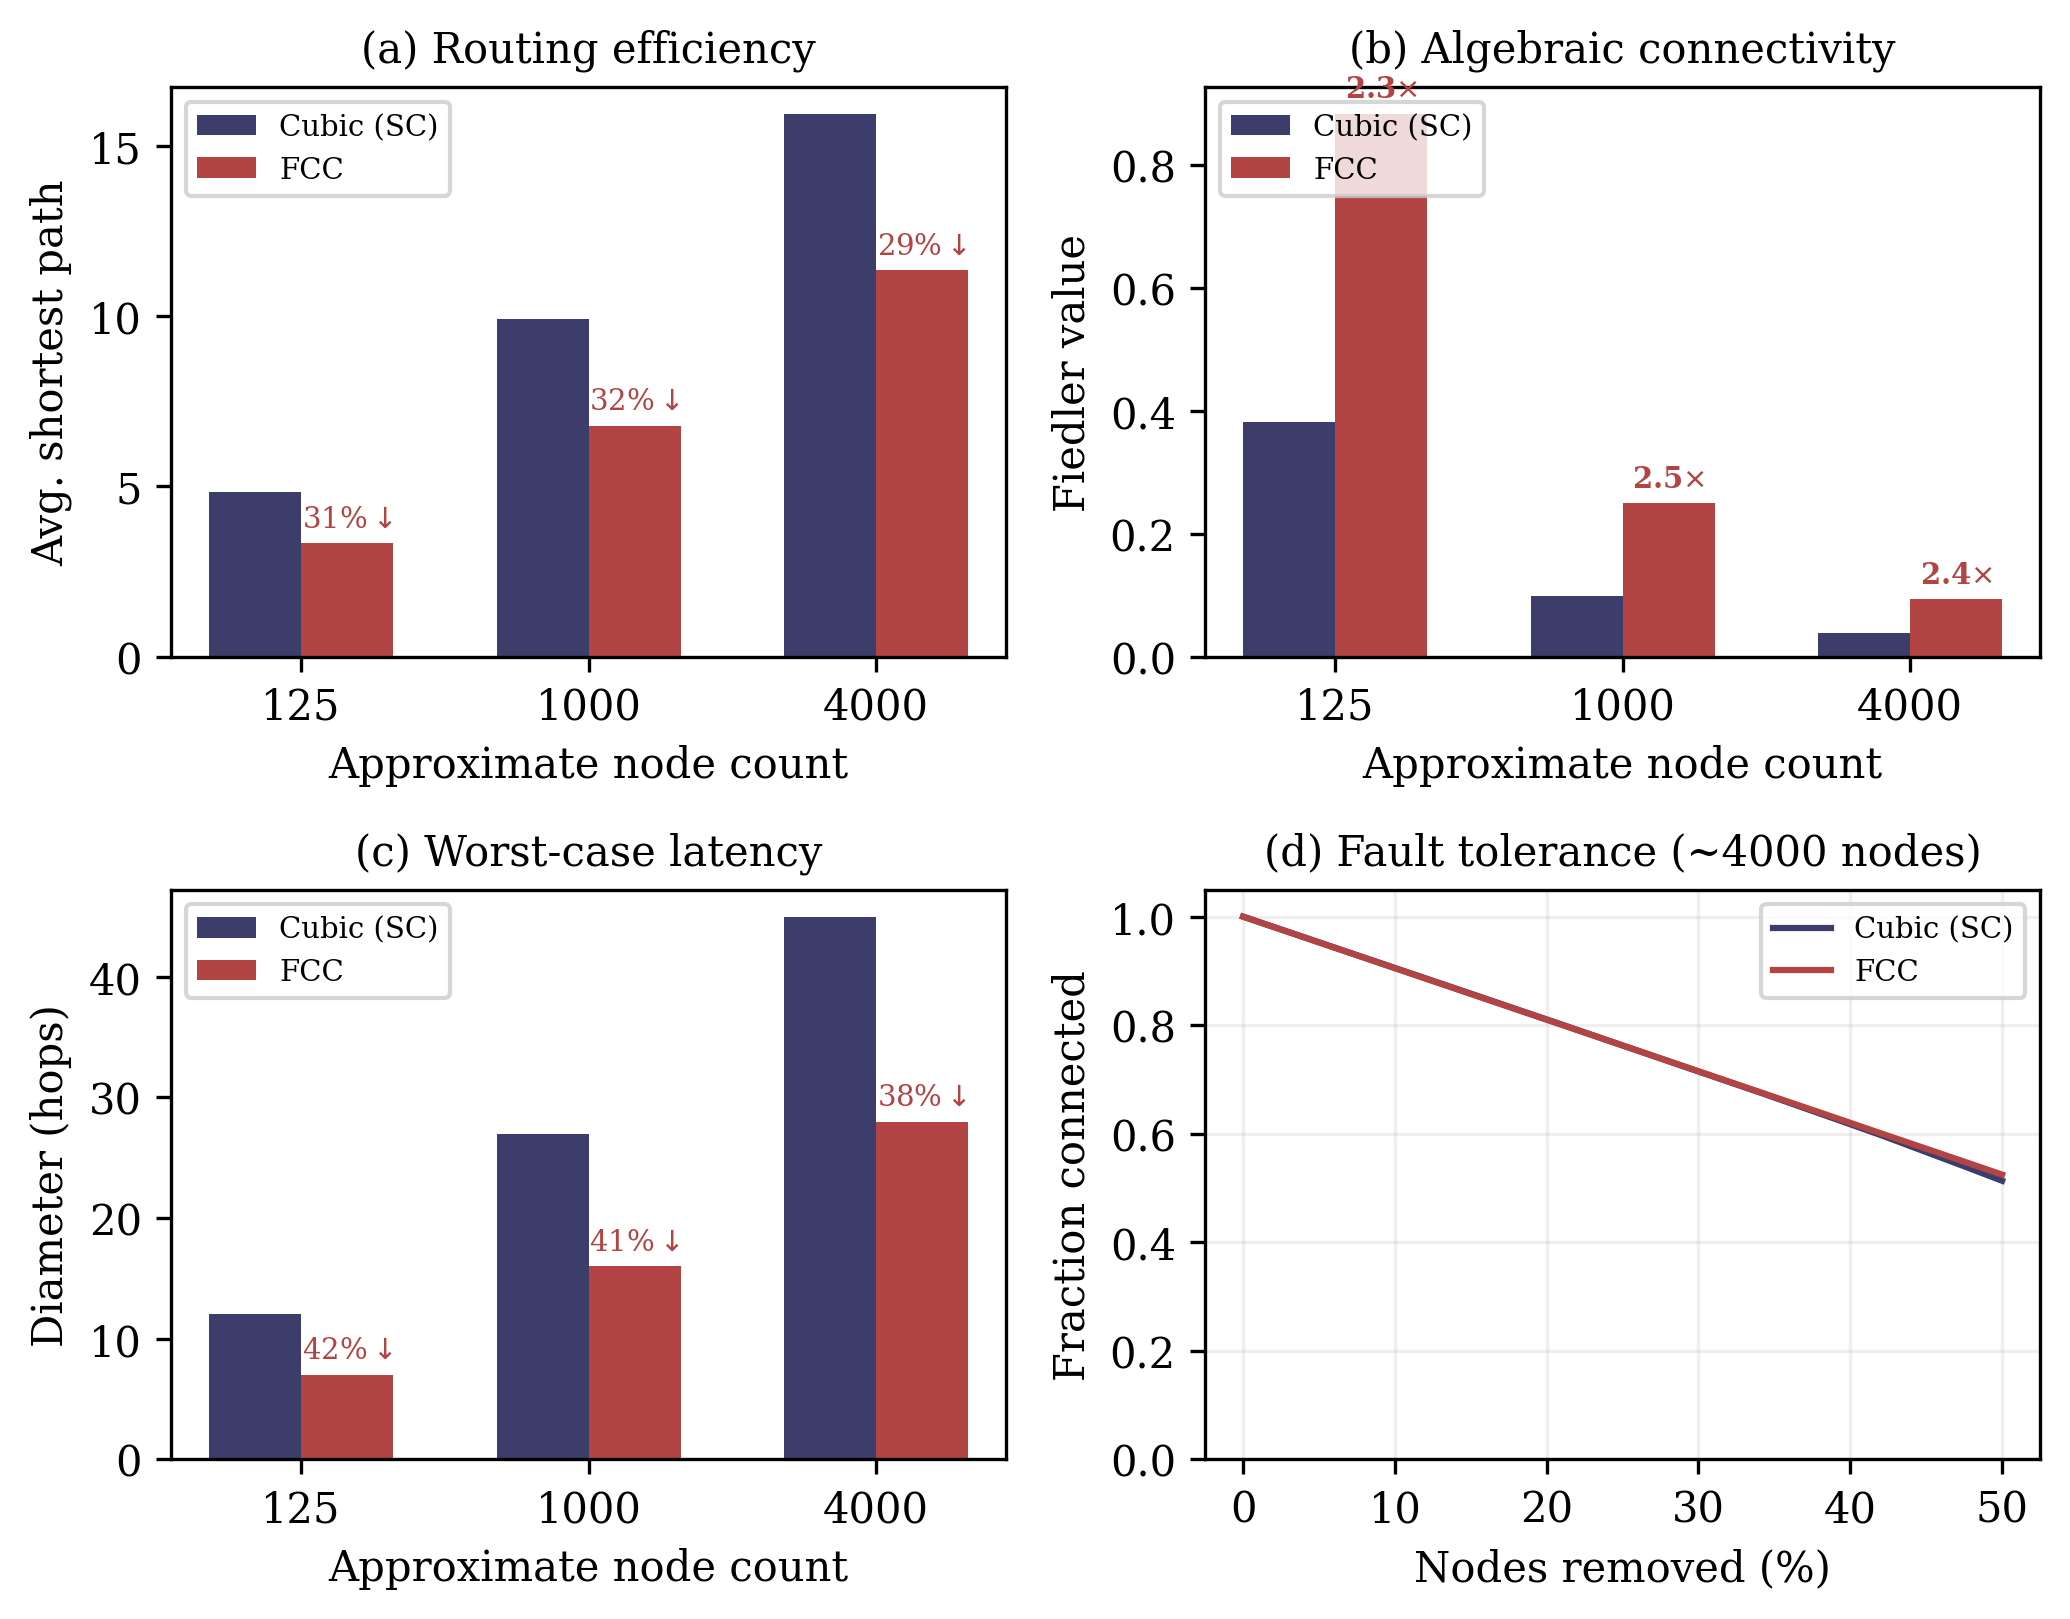
\includegraphics[width=\textwidth]{figures/fig2-graph-benchmarks}
\caption{Benchmark di teoria dei grafi a scala corrispondente. (a)~Lunghezza
  media del cammino minimo: l'FCC riduce i cammini del 29--32\%.
  (b)~Connettivit\`a algebrica (valore di Fiedler): l'FCC raggiunge
  2,3--2,5$\times$ il valore cubico. (c)~Diametro: l'FCC riduce la
  latenza nel caso peggiore del 38--42\%. (d)~Tolleranza ai guasti a
  ${\sim}4{,}000$ nodi: frazione del grafo che rimane connessa man mano
  che i nodi vengono rimossi casualmente.}
\label{fig:benchmarks}
\end{figure}

% ===================================================================
\section{Livello 2: Operazioni spaziali}
\label{sec:spatial}

Cinque operazioni spaziali valutate a tre scale (125--8{,}000
nodi). I nodi del reticolo fungono da punti dati spaziali; le operazioni
utilizzano sia la struttura del grafo sia le coordinate euclidee.

\subsection{Operazioni}

\textbf{Interrogazione del vicino pi\`u prossimo}: interrogazione
a punto singolo con KDTree di SciPy. \textbf{Interrogazione per
sfera/parallelepipedo}: tutti i punti entro un raggio/parallelepipedo
dal punto di interrogazione. \textbf{Flood fill}: BFS da un nodo
centrale, contando i nodi raggiunti a profondit\`a 3.
\textbf{Hash spaziale}: hash basato su griglia con dimensione della cella
$= 2 \times$ la distanza media dal vicino pi\`u prossimo.

\paragraph{Parametri.}
Raggio della sfera = 15\% della diagonale del volume delimitante,
estensione del parallelepipedo = 30\%, 100 interrogazioni casuali per
prova; i tempi riportati escludono il costo di costruzione dell'albero
(incluso nei benchmark del repository).

\subsection{Risultati}

\begin{table}[H]
\centering
\caption{Operazioni spaziali a ${\sim}8{,}000$ nodi
(SC: 8{,}000; FCC: 8{,}788).}
\label{tab:spatial}
\begin{tabular}{lrl}
\toprule
Operazione & FCC vs.\ cubico & Nota \\
\midrule
\multicolumn{3}{l}{\textit{Vantaggi dell'FCC}} \\
Portata flood fill & $+55\%$ & Pi\`u nodi per hop \\
Velocit\`a interr.\ NN & $17\%$ pi\`u veloce & Impacch.\ pi\`u denso, vicini pi\`u prossimi \\
Interr.\ hash spaziale & $6\%$ pi\`u veloce & Celle pi\`u dense \\
Densit\`a interr.\ sfera & $+24\%$ nodi & Pi\`u nodi per volume \\
\midrule
\multicolumn{3}{l}{\textit{Costi dell'FCC}} \\
Tempo interr.\ per intervallo & $3$--$5\times$ pi\`u lento & La densit\`a aumenta il lavoro di scansione \\
\bottomrule
\end{tabular}
\end{table}

I risultati rivelano un chiaro confine decisionale: i carichi di lavoro
\textbf{dominati dalla propagazione} (flood fill, espansione del fronte
d'onda, diffusione dell'influenza) beneficiano in modo inequivocabile
dell'FCC. I carichi di lavoro \textbf{dominati dall'enumerazione}
(interrogazioni per intervallo che scandiscono tutti i nodi in un volume)
pagano un costo di densit\`a proporzionale all'efficienza di
impacchettamento. Le interrogazioni puntuali (NN, ricerca hash) favoriscono
l'FCC poich\'e l'impacchettamento pi\`u denso produce vicini pi\`u
prossimi.

% ===================================================================
\section{Livello 3: Elaborazione del segnale}
\label{sec:signal}

\subsection{Metodo}

Entrambi i reticoli riempiono $[0,1]^3$ con conteggi di campioni a
densit\`a corrispondente. Un segnale di test isotropo
\begin{equation}
  f(\mathbf{x}) = \sin(\omega x)\cos(\omega y)\sin(\omega z)
    + 0.5\cos(\omega r) + 0.3\sin\!\left(\omega\tfrac{x+y+z}{\sqrt{3}}\right)
\end{equation}
dove $r = \|\mathbf{x}\|$ e $\omega = 2\pi f$, viene campionato
ai nodi del reticolo e ricostruito in 600--800 punti di valutazione
casuali tramite interpolazione RBF a piastra sottile (SciPy, smoothing
nullo). Le frequenze spaziano dal 10\% al 100\% della frequenza di
Nyquist cubica.

\subsection{Risultati}

\begin{table}[H]
\centering
\caption{Ricostruzione del segnale: vantaggio massimo dell'FCC
nell'intervallo di frequenza produttivo (10--60\% di Nyquist).}
\label{tab:signal}
\begin{tabular}{rrrr}
\toprule
Campioni & $\Delta$PSNR massimo & Miglior rapporto MSE & Rapporto isotropia \\
\midrule
216   & $+6{,}1$ dB  & $4{,}2\times$ & $0{,}20\times$ \\
512   & $+7{,}3$ dB  & $5{,}3\times$ & $0{,}05\times$ \\
1{,}000 & $+10{,}0$ dB & $10\times$  & $0{,}11\times$ \\
\bottomrule
\end{tabular}
\end{table}

Il vantaggio \emph{cresce con la scala} poich\'e il vantaggio della
regione di Nyquist geometrica ha pi\`u ``spazio'' per esprimersi a
densit\`a di campionamento maggiori. Oltre il limite di Nyquist,
entrambi i reticoli producono aliasing e si osservano casi in cui
l'allineamento agli assi nel reticolo cubico riduce l'errore per le
componenti separabili del segnale. Consideriamo questo come un artefatto
dell'allineamento assiale piuttosto che un vantaggio generale.

La metrica di isotropia (varianza direzionale dell'errore di ricostruzione)
mostra che l'errore di ricostruzione dell'FCC \`e 5--20$\times$ pi\`u
uniforme tra le direzioni. Si tratta di misure empiriche dirette
effettuate con un ricostruttore agnostico rispetto alla topologia, non
di derivazioni dalla teoria del campionamento. Questo approccio di
misura---confrontare la varianza dell'errore direzionale piuttosto che il
solo errore aggregato---pu\`o risultare utile per valutare la qualit\`a
del reticolo indipendentemente dall'argomentazione a favore dell'FCC.

% ===================================================================
\section{Livello 4: Preservazione del vicinato degli embedding}
\label{sec:embed}

\subsection{Metodo}

Generiamo 125--1{,}000 embedding clusterizzati in 128 dimensioni
(5 cluster gaussiani con sovrapposizione). Gli embedding vengono proiettati
in 3D tramite proiezione ortogonale casuale (scelta per evitare bias da
qualsiasi particolare allineamento assiale) e assegnati ai nodi del
reticolo tramite assegnazione al pi\`u prossimo con KDTree. Tre benchmark
misurano quanto la topologia reticolare preserva la struttura di vicinato
ad alta dimensionalit\`a.

\textbf{Recall del vicinato}: frazione dei veri 10 vicini pi\`u prossimi
di un embedding (forza bruta in 128D) catturata dal vicinato a $k$-hop del
suo nodo reticolare. \textbf{Diffusione dell'informazione}: cicli
affinch\'e un impulso di segnale raggiunga il 50\%/80\% del reticolo.
\textbf{Consenso}: cicli di media laplaciana fino alla convergenza
($\epsilon = 0{,}05$).

\subsection{Risultati}

\begin{table}[H]
\centering
\caption{Recall del vicinato a 1-hop e 2-hop.}
\label{tab:recall}
\begin{tabular}{rrrrr}
\toprule
Nodi (SC/FCC) & SC 1-hop & FCC 1-hop & SC 2-hop & FCC 2-hop \\
\midrule
125 / 108   & 0,641 & \textbf{0,903} & 0,932 & \textbf{0,998} \\
512 / 500   & 0,547 & \textbf{0,763} & 0,840 & \textbf{0,971} \\
1000 / 864  & 0,508 & \textbf{0,658} & 0,756 & \textbf{0,915} \\
\bottomrule
\end{tabular}
\end{table}

A 1-hop, l'FCC cattura 15--26 punti percentuali in pi\`u di veri
vicini pi\`u prossimi. L'informazione si diffonde 1,4--2$\times$ pi\`u
velocemente. Il consenso converge 1,58$\times$ pi\`u rapidamente a 500
nodi, sebbene la diluizione del peso per vicino ($1/13$ contro $1/7$)
riduca il vantaggio a 1{,}000 nodi (0,93$\times$).

% ===================================================================
\section{Indice di embedding FCC}
\label{sec:index}

Per verificare se il vantaggio topologico persiste in un carico di
lavoro di recupero realistico, implementiamo un indice ANN come prova
di concetto.

\subsection{Architettura}

\begin{enumerate}
  \item \textbf{Proiettare} gli embedding da $d$ dimensioni a 3D tramite
    PCA (deterministica, preserva la varianza massima). La PCA \`e
    utilizzata qui, anzich\'e la proiezione randomizzata del Livello~4,
    poich\'e una pipeline di recupero pratica proietterebbe tipicamente
    lungo le direzioni di varianza massima. (La PCA \`e lineare;
    proiezioni non lineari potrebbero produrre recall assoluta differente,
    ma il confronto topologico rimane valido poich\'e entrambi i reticoli
    ricevono embedding identici.)
  \item \textbf{Quantizzare} ai nodi del reticolo tramite assegnazione al
    pi\`u prossimo con KDTree.
  \item \textbf{Memorizzare} i vettori originali a $d$ dimensioni nei
    nodi assegnati.
  \item \textbf{Interrogare} proiettando la query in 3D, trovando il suo
    nodo reticolare, raccogliendo tutti i vettori dal vicinato a $k$-hop
    e classificandoli per similarit\`a coseno nello spazio originale.
\end{enumerate}

Sia \texttt{FCCIndex} che \texttt{CubicIndex} condividono la stessa
classe base \texttt{LatticeIndex}. La differenza architetturale tra essi
\`e il pattern di connettivit\`a (sebbene anche i conteggi effettivi dei
nodi differiscano leggermente; Tabella~\ref{tab:index}).

\subsection{Risultati}

\begin{table}[H]
\centering
\caption{Recall@10 su embedding sintetici (384D, 30 cluster
sovrapposti, 1{,}800 vettori nel corpus, 200 interrogazioni). Verit\`a
di base tramite similarit\`a coseno a forza bruta.}
\label{tab:index}
\begin{tabular}{rllrrr}
\toprule
Obiettivo & Topologia & Effettivi & 1-hop & 2-hop & 3-hop \\
\midrule
125  & Cubico       & 125 & 0,379 & 0,788 & 0,999 \\
125  & \textbf{FCC}& 108 & \textbf{0,445} & \textbf{0,971} & \textbf{1,000} \\
\midrule
500  & Cubico       & 512 & 0,085 & 0,324 & 0,551 \\
500  & \textbf{FCC}& 500 & \textbf{0,280} & \textbf{0,488} & \textbf{0,789} \\
\midrule
1000 & Cubico       & 1000 & 0,044 & 0,138 & 0,414 \\
1000 & \textbf{FCC}& 864 & \textbf{0,216} & \textbf{0,349} & \textbf{0,616} \\
\bottomrule
\end{tabular}
\end{table}

L'indice FCC raggiunge +7--20 punti percentuali di recall in pi\`u
a 1-hop a tutte le scale. A 500 nodi obiettivo, il divario \`e massimo:
28,0\% contro 8,5\%, un miglioramento relativo di 3,3$\times$.
Il vantaggio \`e coerente con la differenza di connettivit\`a, poich\'e
le procedure di proiezione, assegnazione e classificazione sono identiche.
Tuttavia, la discrepanza nel conteggio dei nodi
(Tabella~\ref{tab:index}) pu\`o anch'essa contribuire; un controllo a
conteggio corrispondente \`e indicato come lavoro futuro. Il vantaggio
dell'FCC \`e coerente con entrambi i metodi di proiezione (ortogonale
casuale nel Livello~4, PCA nella Sezione~\ref{sec:index}), suggerendo
che l'effetto topologico \`e robusto rispetto alla scelta della
proiezione.

% ===================================================================
\section{Discussione}
\label{sec:discussion}

\subsection{Il pattern}

Le interpretazioni seguenti sono coerenti con le misure sopra riportate;
si tratta di ipotesi sui meccanismi, non di dimostrazioni di causalit\`a.

In tutti e quattro i domini emerge un pattern coerente:

\textbf{La propagazione prevale.} Qualsiasi carico di lavoro in cui
l'informazione si propaga attraverso il reticolo---instradamento,
flooding, diffusione, ricostruzione del segnale, recupero del
vicinato---beneficia della topologia FCC. La struttura 12-connessa
propaga pi\`u velocemente, pi\`u lontano e in modo pi\`u isotropo
rispetto alla 6-connessa.

\textbf{L'isotropia prevale.} I 12 vicini del reticolo FCC coprono le
direzioni in modo uniforme. I 6 vicini del reticolo cubico coprono
soltanto gli assi coordinati. Per compiti senza una direzione
privilegiata (similarit\`a degli embedding, larghezza di banda del
segnale, propagazione dei guasti), l'isotropia \`e la geometria
superiore.

\textbf{L'enumerazione ha un costo.} Le interrogazioni per intervallo
che devono scandire tutti i nodi in una regione pagano un costo di
densit\`a proporzionale all'efficienza di impacchettamento
(${\sim}1{,}24\times$ nodi in pi\`u per volume, scanditi
$3$--$5\times$ pi\`u lentamente).

\subsection{Invarianza di scala}

I rapporti riportati nelle
Sezioni~\ref{sec:graph}--\ref{sec:embed} sono stabili a tutte le scale
testate (125--8{,}000 nodi). Questa stabilit\`a suggerisce un'origine
geometrica: a scale ben al di sopra dello strato di bordo, i rapporti
sono determinati dal numero di coordinazione (12 contro 6), dalla
configurazione del kissing number e dalla forma della cella di
Voronoi---costanti del reticolo, non funzioni della dimensione del
campione. Se questa stabilit\`a si estenda a scale oltre quelle qui
testate \`e una questione empirica per il lavoro futuro.

\subsection{Il costo}

Il reticolo FCC utilizza approssimativamente $2\times$ pi\`u archi
rispetto al reticolo SC a conteggi di nodi corrispondenti
(asintoticamente esatto: $12/6 = 2$). La Tabella~\ref{tab:cost}
contestualizza questo costo nei diversi domini.

\begin{table}[H]
\centering
\caption{Costo del $2\times$ di archi nei diversi domini.}
\label{tab:cost}
\begin{tabular}{lll}
\toprule
Dominio & Costo degli archi & $2\times$ archi significa \\
\midrule
Rete fisica & Fili, tracce, alimentazione & Vincolo reale \\
Struttura software & Puntatore da 8 byte & ${\sim}$96 vs.\ 48 byte/nodo \\
Topologia logica & Nulla finch\'e non attraversata & Arrivo il 30\% prima \\
Indice di embedding & Un candidato da valutare & +7--20pp di recall \\
Campionamento del segnale & Una misurazione & Fedelt\`a 4--10$\times$ migliore \\
\bottomrule
\end{tabular}
\end{table}

I domini in cui il costo \`e proibitivo (interconnessioni su chip) sono
quelli in cui il vantaggio conta di pi\`u. I domini in cui il costo \`e
trascurabile (software, topologia logica) sono quelli in cui l'adozione
\`e pi\`u agevole.

\subsection{Interpretazione cibernetica}

Le connessioni seguenti sono interpretative, non empiriche; suggeriscono
perch\'e i vantaggi misurati si manifestano ma non costituiscono prove
indipendenti.

La legge della variet\`a necessaria di Ashby~\cite{ashby1956} predice il
risultato di connettivit\`a algebrica: un sistema deve eguagliare la
variet\`a delle perturbazioni che affronta. Una cella 12-connessa assorbe
perturbazioni lungo 12 direzioni; l'isotropia amplifica oltre il semplice
rapporto di grado $2\times$ producendo una connettivit\`a algebrica
$2{,}3$--$2{,}5\times$. Il Modello di Sistema Vitale di
Beer~\cite{beer1972} distingue le gerarchie fragili (facilmente
partizionabili lungo gli assi) dai sistemi vitali (cammini ridondanti
resistono alla frammentazione). Il reticolo SC \`e allineato agli assi e
fragile lungo gli assi; il reticolo FCC \`e isotropo e robusto.

\subsection{Quando il reticolo cubico prevale}

Il reticolo SC mantiene vantaggi pratici in diversi scenari.
\textbf{Layout di memoria:} l'indirizzamento cubico si mappa direttamente
sulla memoria lineare tramite $i + jN + kN^2$, consentendo la
vettorizzazione SIMD e pattern di accesso allineati alle linee di cache
che l'indirizzamento FCC compromette. \textbf{Interrogazioni per
intervallo:} a 8{,}000 nodi, le interrogazioni per sfera e
parallelepipedo sull'FCC sono 3--5$\times$ pi\`u lente
(Tabella~\ref{tab:spatial}) poich\'e l'impacchettamento pi\`u denso
produce pi\`u candidati da scandire. \textbf{Consenso su larga scala:}
la media laplaciana sull'FCC converge pi\`u lentamente rispetto all'SC a
1{,}000 nodi (0,93$\times$) a causa della diluizione del peso per vicino
($1/13$ contro $1/7$). \textbf{Carichi di lavoro allineati agli assi:}
quando il segnale o il pattern di accesso \`e intrinsecamente allineato
agli assi (filtri separabili, scansioni rettilinee), l'allineamento
coordinato del reticolo SC \`e un vantaggio, non una limitazione.

\subsection{Limitazioni e minacce alla validit\`a}

\textbf{Solo tre dimensioni.} Questi risultati sono specifici per i
reticoli 3D. L'estensione a dimensioni superiori (D$_4$ in 4D, $E_8$ in
8D, reticolo di Leech in 24D) \`e lavoro futuro.

\textbf{Indice a prova di concetto.} L'indice di embedding FCC non
\`e competitivo con i sistemi ANN di produzione (HNSW, IVF-PQ). Esiste
per isolare la variabile topologica, non per proporre un'architettura di
produzione.

\textbf{Nessun modello nullo formale.} Confrontiamo l'FCC con l'SC
direttamente. Un'analisi formale che decomponga il vantaggio in componenti
attribuibili al grado e all'isotropia rafforzerebbe il contributo teorico.

\textbf{Tolleranza ai guasti mirata.} Abbiamo testato la rimozione
casuale dei nodi. Sotto attacco mirato (rimozione dei nodi ad alta
betweenness), il vantaggio dell'FCC dovrebbe essere pi\`u marcato.

\textbf{Benchmark a singola prova.} I benchmark del segnale e degli
embedding utilizzano una singola prova per configurazione con seme fisso.
Sebbene i risultati deterministici siano esattamente riproducibili,
intervalli di confidenza da semi multipli rafforzerebbero le asserzioni
statistiche.

\textbf{Intervallo di scala.} Tutti i benchmark operano tra 125 e 8{,}000
nodi. La stabilit\`a dei rapporti in questo intervallo \`e coerente con
un'origine geometrica, ma l'estrapolazione oltre le scale testate non \`e
verificata empiricamente.

% ===================================================================
\section{Conclusione}
\label{sec:conclusion}

Per i carichi di lavoro isotropi e dominati dalla propagazione qui
testati, il reticolo SC \`e costantemente superato. In quattro domini
indipendenti e quattro livelli sperimentali, il reticolo FCC offre
vantaggi misurabili e riproducibili che sono stabili a tutte le scale
testate. Il costo \`e limitato (${\sim}2\times$ archi) e il beneficio si
accumula (30\% instradamento $+$ 55\% propagazione $+$ 4--10$\times$
fedelt\`a del segnale $+$ 15--26pp recall del vicinato).

Il reticolo FCC (con l'HCP) realizza l'impacchettamento sferico pi\`u
denso e la topologia che le strutture naturali a impacchettamento denso
comunemente esibiscono. Il reticolo SC persiste nel calcolo in gran parte
per convenzione piuttosto che per ottimalit\`a dimostrata nei carichi di
lavoro isotropi. Questa libreria e questo articolo forniscono la base
quantitativa per riconsiderare tale eredit\`a. Per i professionisti che
valutano la topologia reticolare nei propri domini, raccomandiamo di
misurare direttamente:
\texttt{pip install rhombic \&\& python -m rhombic.benchmark}.

\paragraph{Disponibilit\`a.}
Codice sorgente: \url{https://github.com/promptcrafted/rhombic}.\\
Pacchetto: \url{https://pypi.org/project/rhombic/}.\\
Demo interattiva: \url{https://huggingface.co/spaces/timotheospaul/rhombic}.

% ===================================================================
\section*{Ringraziamenti}

L'autore ringrazia Araminta K per la collaborazione in Promptcrafted, e
la cibernetica di Ashby, Beer e Bateson per il framework interpretativo.
Porzioni del codice e del manoscritto sono state sviluppate con
l'assistenza di intelligenza artificiale (Claude, Anthropic).

% ===================================================================
\bibliographystyle{plainnat}
\bibliography{rhombic}

\end{document}
